%% LyX 2.0.6 created this file.  For more info, see http://www.lyx.org/.
%% Do not edit unless you really know what you are doing.
\documentclass[english]{article}
\usepackage[T1]{fontenc}
\usepackage[latin9]{inputenc}
\usepackage{geometry}
\geometry{verbose,tmargin=1cm,bmargin=2cm,lmargin=2.5cm,rmargin=2.5cm,headheight=1cm,headsep=1cm,footskip=1.5cm}
\setlength{\parindent}{0bp}
\usepackage{babel}
\usepackage{float}
\usepackage{amssymb}
\usepackage{graphicx}
\usepackage{setspace}
\PassOptionsToPackage{normalem}{ulem}
\usepackage{ulem}
\usepackage[unicode=true,
 bookmarks=true,bookmarksnumbered=false,bookmarksopen=false,
 breaklinks=false,pdfborder={0 0 1},backref=false,colorlinks=false]
 {hyperref}


%%%%%%%%%% Easily edit these definitions:
\def\LabNumber{II}
\def\year{2013}
%%%%%%%%%%
\hypersetup{pdftitle={Lab Exercise \LabNumber: Introduction to Binary Stars},
 pdfauthor={Amit Vishwas},
 pdfsubject={Astronomy 1103}}




\makeatletter

%%%%%%%%%%%%%%%%%%%%%%%%%%%%%% LyX specific LaTeX commands.
%% Because html converters don't know tabularnewline
\providecommand{\tabularnewline}{\\}

\makeatother

\begin{document}
\begin{table}[H]
\begin{doublespace}
\begin{centering}
\uline{Lab \LabNumber ~~~~~~~~~~~~~~~~~~~~~~~~~~~~~~~~~~~~~~~~~~~~~~~~
Fall \year ~~~~~~~~~~~~~~~~~~~~~~~~~~~~~
Astro 1103 - Nature of the Universe}
\par\end{centering}
\end{doublespace}

\centering{}%
\begin{tabular}{lclc}
 &  &  & \tabularnewline
Name: & ~~~~~~~~~~~~~~~~~~~~~~~~~~~~~~~~~~~~~~~~~~ & Partner(s): & ~~~~~~~~~~~~~~~~~~~~~~~~~~~~~~~~~~~~~~~~~~~~~~~~\tabularnewline
 &  &  & \tabularnewline
Student ID\#: &  & Date: & \tabularnewline
\end{tabular}
\end{table}


\vspace{0.15in}


\begin{center}
{\LARGE{Lab Exercise \LabNumber : Introduction to Binary Stars}}
\par\end{center}{\LARGE \par}

\medskip{}




\section{Purpose}

To allow you to investigate the orbital properties of binary star systems and how the masses of stars are determined.


\section{Introduction to Binary Stars}

One of the fundamental properties that we want to know about a star is its mass. The only way that we can determine the masses of stars is to study the orbital motions of binary stars. Application of the
laws of celestial mechanics allows us to calculate the masses of the stars from measures of their orbital periods, sizes and velocities.

\smallskip{}


Five to ten percent of the stars visible to us are visual binaries. Careful spectroscopic studies of nearby solar-type stars show that about two thirds of them have stellar companions. We estimate that
roughly half of all stars in the sky are indeed members of binaries.

\smallskip{}

% % Add location of the python program here
Using the Orbit Simulator available on the lab computer, we will experiment with many of the observable properties of binary star systems.

\smallskip{}
\pagebreak{}

\begin{doublespace}
\begin{center}
\uline{Lab \LabNumber ~~~~~~~~~~~~~~~~~~~~~~~~~~~~~~~~~~~~~~~~~~~~~~~~
Fall \year ~~~~~~~~~~~~~~~~~~~~~~~~~~~~~
Astro 1103 - Nature of the Universe}
\par\end{center}
\end{doublespace}


\section{Binary Stars}


\subsection{Mass Ratios and the Center of Mass }

Start with the eccentricity and inclination set to zero. Do this by dragging the sliders labeled \textit{Ecc} and \textit{Inc} to 0. Since a circle is just an ellipse with eccentricity equal to zero, that means that the orbits are circular.
Set the mass of each body to be equal to 1 (sliders $m_{1}$ and $m_{2}$ each show masses in units of solar mass, $M_{\circledcirc}$). For $m_{1}=m_{2}$, the ratio, $\frac{m_{1}}{m_{2}}$, is one. Now vary the mass ratio. When the mass ratio is greater than one, the red star (with mass $m_{1}$) is more massive and the blue one (with mass $m_{2}$) is the less massive. Answer the following Questions:

\vspace{0.2in}

\begin{enumerate}
\item Vary the Mass Ratio

\begin{enumerate}
\item What happens to the orbit of the more massive star as the ratio of the masses $\frac{m_{1}}{m_{2}}$ grows?
\end{enumerate}

\rule[0.5pt]{0.75\paperwidth}{0.3pt}\vspace{0.2in}
\rule[0.5pt]{0.75\paperwidth}{0.3pt}\vspace{0.1in}


\item Let\textquoteright{}s digress from the simulator for a moment. Assume we have observations of two binary star systems. In both systems,
the orbital period is eight years. For one system, the mass ratio is one; for the other, it is three. Using the Kepler\textquoteright{}s Third Law, calculate the semimajor axis in each system?

\begin{enumerate}
\item \textbf{Binary \#1:} P = 8 yr , $m_{1}=m_{2}$ = 1 $M_{\circledcirc}$ , a = \rule[0.5pt]{0.05\paperwidth}{0.3pt} AU\vspace{0.2in}

\item \textbf{Binary \#2:} P = 8 yr , $m_{1}=3m_{2}$; $m_{2}$ = 1 $M_{\circledcirc}$
, a = \rule[0.5pt]{0.05\paperwidth}{0.3pt} AU
\end{enumerate}

Based on your calculations, how does the semimajor axis change with varying mass ratio for binaries with the same period and $m_{2}$ fixed?


\vspace{0.1in}



\rule[0.5pt]{0.75\paperwidth}{0.3pt}\vspace{0.1in}


\item The Sun is about 1000 times more massive than Jupiter, the most massive of the planets. Is the center of mass of the Solar System closer to the Sun or to Jupiter?


\rule[0.5pt]{0.75\paperwidth}{0.3pt}\vspace{0.1in}



\rule[0.5pt]{0.75\paperwidth}{0.3pt}\vspace{0.2in}


\end{enumerate}
\pagebreak{}

\begin{doublespace}
\begin{center}
\uline{Lab II ~~~~~~~~~~~~~~~~~~~~~~~~~~~~~~~~~~~~~~~~~~~~~~~~
Fall \year ~~~~~~~~~~~~~~~~~~~~~~~~~~~~~
Astro 1103 - Nature of the Universe}
\par\end{center}
\end{doublespace}


\subsection{Eccentricity }

Notice that you can change the eccentricity from 0 to 0.9. Highly eccentric orbits are very rare in nature. In the Solar System, most of the planets
follow almost circular orbits. The eccentricity of the Earth\textquoteright{}s orbit is 0.0167; the most eccentric of the planetary orbits is that of Pluto with e = 0.2484. Now, answer the following questions:

\vspace{0.2in}

\begin{enumerate}
\item Set the mass ratio to 100:1 and the eccentricity to 0. Watch the orbit. Then change the eccentricity to 0.1, 0.2, 0.3 and 0.4 and, each time,
watch what happens to the orbits. We can now define two extreme points on the less massive star\textquoteright{}s orbit. \textbf{Periastron}
occurs when the two stars are closest together. \textbf{Apastron} occurs when the two stars are furthest apart. In the space below, sketch the case for $e=0.3$ and label on your sketch the locations
of \textbf{Periastron} and \textbf{Apastron}. Also, label the locations of the two stars $m_{1}$ and $m_{2}$ and the center of mass. (Tip: You can pause the motion of the stars by clicking anywhere on the window)

\begin{enumerate}
\item Case: $m_{1}=100m_{2}$ , $e=0.3$
\end{enumerate}

\rule[0.5pt]{0.75\paperwidth}{0.3pt}


\vspace{1in}


\item Leave the eccentricity at 0.3. Now set the mass ratio to 1:1. Again, sketch below the orbits of the two stars. Indicate where the two stars
will be when $m_{1}$ is at periastron. Locate and label the center of mass.

\begin{enumerate}
\item Case: $m_{1}=m_{2}$ , $e=0.3$
\end{enumerate}

\rule[0.5pt]{0.75\paperwidth}{0.3pt}


\vspace{1in}


\item When the blue star is at periastron, where is the red star in its orbit?


\vspace{0.1in}
\rule[0.5pt]{0.75\paperwidth}{0.3pt}\vspace{0.1in}

\begin{enumerate}
\item When the blue star is at apastron, where is the red star in its orbit?


\vspace{0.1in}
\rule[0.5pt]{0.7\paperwidth}{0.3pt}\vspace{0.1in}


\item What can you say about the distances of the two stars from the center of mass at periastron?


\vspace{0.1in}
\rule[0.5pt]{0.7\paperwidth}{0.3pt}\vspace{0.1in}


\end{enumerate}

\pagebreak{}


\uline{\hspace{-0.4in}Lab \LabNumber ~~~~~~~~~~~~~~~~~~~~~~~~~~~~~~~~~~~~~~~~~~~~~~~~
Fall \year ~~~~~~~~~~~~~~~~~~~~~~~~~~~~~
Astro 1103 - Nature of the Universe}\vspace{0.3in}


\item Now change the mass ratio to 3:1. Sketch the orbit below. Show the two stars\textquoteright{} locations at apastron. Mark the center of mass.

\begin{enumerate}
\item Case: $m_{1}=3m_{2}$ , $e=0.3$
\end{enumerate}

\rule[0.5pt]{0.75\paperwidth}{0.3pt}


\vspace{1in}


\item Watch the less massive star. Does it travel at the same speed at all points in its orbit?


\vspace{0.1in}
\rule[0.5pt]{0.75\paperwidth}{0.3pt}
\begin{enumerate}
\item When does it travel fastest?


\vspace{0.1in}
\rule[0.5pt]{0.7\paperwidth}{0.3pt}\vspace{0.1in}


\item Which of Kepler\textquoteright{}s laws predicts this? Explain.


\vspace{0.1in}
\rule[0.5pt]{0.7\paperwidth}{0.3pt}\vspace{0.1in}
\rule[0.5pt]{0.7\paperwidth}{0.3pt}\vspace{0.1in}


\item If the orbit were circular, what can you say about periastron and apastron?


\vspace{0.1in}
\rule[0.5pt]{0.7\paperwidth}{0.3pt}\vspace{0.1in}
\rule[0.5pt]{0.7\paperwidth}{0.3pt}\vspace{0.1in}


\item Does the speed of the bodies change in the same way as when eccentricity is set to e = 0.3?


\vspace{0.1in}
\rule[0.5pt]{0.7\paperwidth}{0.3pt}\vspace{0.1in}
\rule[0.5pt]{0.7\paperwidth}{0.3pt}\vspace{0.1in}


\end{enumerate}
\end{enumerate}

\subsection{Inclination}

Up until now, we have been viewing orbits that lie flat in the plane of the computer screen. In our simulation, the screen is like the plane of the sky. Of course, real binary star systems can orbit in
planes that have any orientation with respect to the plane of sky as viewed from the Earth, and so we have to introduce another variable:
the \textbf{\textit{Inclination}} of the true orbit with respect to the sky. According to convention, the inclination is zero degrees when the orbit is flat in the plane of the sky, i.e., perpendicular
to our line of sight. When the orbit is inclined 90 degrees with respect to the plane of the sky, it lies in a plane aligned with the line of sight. So far, we have only dealt with the $0^{\circ}$ case. Notice the \textit{Top View} available on the top-left of the screen.
It allows you to view the orbit from the top down, as if it were flat in the plane of the sky, no matter what the inclination is.

\vspace{0.1in}


When the inclination is $90^{\circ}$, a star passing exactly in front of its companion may block out the light we see from the companion. When this happens, we say that the companion is eclipsed, and the
system is called an \textbf{Eclipsing Binary}. For such eclipses to be seen, the inclination must be close to or exactly $90^{\circ}$. Lets try answering the questions on the next page.

\pagebreak{}

\begin{doublespace}
\begin{center}
\uline{Lab \LabNumber ~~~~~~~~~~~~~~~~~~~~~~~~~~~~~~~~~~~~~~~~~~~~~~~~
Fall \year ~~~~~~~~~~~~~~~~~~~~~~~~~~~~~
Astro 1103 - Nature of the Universe}
\par\end{center}
\end{doublespace}

\vspace{0.2in}

\begin{enumerate}
\item Set the mass ratio equal to 3:1 and the eccentricity equal to zero.
Remind yourself of what the orbit should look like; this is the true orbit of the system. Now vary the inclination angle. What happens to a true circular orbit when it is viewed with a non-zero inclination
angle?


\vspace{0.1in}
\rule[0.5pt]{0.7\paperwidth}{0.3pt}\vspace{0.1in}



\rule[0.5pt]{0.7\paperwidth}{0.3pt}\vspace{0.1in}


\item Now set the eccentricity equal to 0.3 and the inclination angle to $45^{\circ}$. Watch both the view as seen by Observer and the \textquotedbl{}Top view\textquotedbl{} (on the top-left). The top
view is the true orbit. In the space below, sketch both views.

\begin{enumerate}
\item Case: $m_{1}=3m_{2}$ , $e=0.3$ , $i=45^{\circ}$
\end{enumerate}

\rule[0.5pt]{0.75\paperwidth}{0.3pt}


\vspace{1in}


\end{enumerate}
\textbf{True Orbit - Apparent Orbit}

\vspace{0.1in}

\begin{enumerate}
\item [3.]\setcounter{enumi}{3}How does the distance from either star to the center of mass at apastron vary as the inclination changes? (Tip: Click anywhere on the window to pause the simulation)


\vspace{0.1in}
\rule[0.5pt]{0.7\paperwidth}{0.3pt}\vspace{0.1in}



\rule[0.5pt]{0.7\paperwidth}{0.3pt}\vspace{0.1in}


\item Now set the inclination to $90^{\circ}$. Sketch the apparent orbit.

\begin{enumerate}
\item Case: $m_{1}=3m_{2}$ , $e=0.3$ , $i=90^{\circ}$
\end{enumerate}

\rule[0.5pt]{0.75\paperwidth}{0.3pt}


\vspace{1in}


\item Set the inclination to $30^{\circ}$. Sketch the apparent orbit.

\begin{enumerate}
\item Case: $m_{1}=3m_{2}$ , $e=0.0$ , $i=30^{\circ}$
\end{enumerate}

\rule[0.5pt]{0.75\paperwidth}{0.3pt}


\vspace{1in}


\end{enumerate}
\pagebreak{}

\begin{doublespace}
\begin{center}
\uline{Lab \LabNumber ~~~~~~~~~~~~~~~~~~~~~~~~~~~~~~~~~~~~~~~~~~~~~~~~
Fall \year ~~~~~~~~~~~~~~~~~~~~~~~~~~~~~
Astro 1103 - Nature of the Universe}
\par\end{center}
\end{doublespace}

\vspace{-0.1in}
\subsection{Radial Velocity}

The radial velocity is the speed of the star towards or away from us, that is, along our line of sight to the star. In the simulator program, set $m_{1}=3m_{2}$ and eccentricity, $ecc = 0$ and inclination, $Inc = 90^{\circ}$

\vspace{0.1in}


During each orbital period, each star has to travel around its orbit once. Since the orbital period of each is the same but the distance each star must travel in order to make one circuit of its orbit is
different, the speed of travel is different for the two stars.

\vspace{0.1in}


Notice that when we measure the maximum radial velocity, also referred to as the \textit{amplitude of the radial velocity} curve and designated
$K$, we really measure the true velocity $V$ modified by the inclination:
$V\, sin\,(i)$. Answer the following questions now: 

\vspace{0.1in}

\begin{enumerate}
\item Which star has the greatest maximum radial velocity, the more massive star or the less massive one?


\vspace{0.1in}
\rule[0.5pt]{0.7\paperwidth}{0.3pt}\vspace{0.1in}

\begin{enumerate}
\item Now vary the mass ratio and look at the maximum radial velocities of the two stars in each case. What happens when the mass ratio is
one: $m_{1}=m_{2}$?


\vspace{0.1in}
\rule[0.5pt]{0.7\paperwidth}{0.3pt}\vspace{0.1in}



\rule[0.5pt]{0.7\paperwidth}{0.3pt}\vspace{0.1in}


\item What can you say in general about how the radial velocities of the two stars compare depending on their mass ratio?


\vspace{0.1in}
\rule[0.5pt]{0.7\paperwidth}{0.3pt}\vspace{0.1in}



\rule[0.5pt]{0.7\paperwidth}{0.3pt}\vspace{0.1in}


\end{enumerate}
\item {}

\begin{enumerate}
\item Set the mass ratio to 3:1, the eccentricity to 0, and the inclination to $30^{\circ}$. Sketch the results and properly label the axis. Show how the velocity varies during two orbital periods. Be sure to indicate which is the curve for the less massive star and which is for the more massive one.


\vspace{0.1in}
\rule[0.5pt]{0.7\paperwidth}{0.3pt}\vspace{1in}



\rule[0.5pt]{0.7\paperwidth}{0.3pt}\vspace{0.1in}


\item You found in \textbf{\textit{Section 3.2 - Q5}} the location in the orbit when the star travels fastest. In the case you are displaying now, what can you say about the apparent speed of the blue star? Is it actually traveling fastest when its radial velocity is most positive? Justify your answers with a short argument.


\vspace{0.1in}
\rule[0.5pt]{0.7\paperwidth}{0.3pt}\vspace{0.1in}



\rule[0.5pt]{0.7\paperwidth}{0.3pt}\vspace{0.1in}


\end{enumerate}
\item Now change the eccentricity to 0.3, 0.5, and 0.7. What happens to the radial velocity of the blue star as the eccentricity changes? Explain why this happens.


\vspace{0.1in}
\rule[0.5pt]{0.7\paperwidth}{0.3pt}\vspace{0.1in}



\rule[0.5pt]{0.7\paperwidth}{0.3pt}\pagebreak{}


\uline{\hspace{-0.4in}Lab \LabNumber ~~~~~~~~~~~~~~~~~~~~~~~~~~~~~~~~~~~~~~~~~~~~~~~~
Fall \year ~~~~~~~~~~~~~~~~~~~~~~~~~~~~~
Astro 1103 - Nature of the Universe}\vspace{0.3in}


\item Set the eccentricity back to 0 and set the inclination to $0^{\circ}$. What does the radial velocity curve look like? Why?


\vspace{0.1in}
\rule[0.5pt]{0.7\paperwidth}{0.3pt}\vspace{0.8in}



\rule[0.5pt]{0.7\paperwidth}{0.3pt}\vspace{0.1in}


\item Set the eccentricity to 0.3. Now change the inclination to $30^{\circ}$, $45^{\circ}$, $60^{\circ}$ and $90^{\circ}$. In comparison with
what you did in Q3 above, which is more critical in making the radial velocity curve change, the inclination or the eccentricity?


\vspace{0.1in}
\rule[0.5pt]{0.7\paperwidth}{0.3pt}\vspace{0.8in}



\rule[0.5pt]{0.7\paperwidth}{0.3pt}\vspace{0.1in}


\end{enumerate}

\subsection{Node Angle }

The last important parameter is the orientation of the major axis of the binary relative to the line of sight, or what we call the \textbf{Node Angle}. When the node angle is set to zero the two stars are lined
up in the horizontal direction. The display shows both the top view and the view as seen by the observer. You can change the node angle by adjusting
the $Node Angle$ slider. Now set the mass ratio to 3, eccentricity to 0.5 and inclination to 0. Change the node angle to $-45^{\circ}$, $45^{\circ}$, etc. You will see what we mean by node angle. Leave the inclination at $0^{\circ}$ and return the node
angle to $0^{\circ}$. 

\vspace{0.1in}


The node angle is probably the hardest concept to visualize, but we hope that this demonstration will help. When the node angle and inclination
are both $0^{\circ}$, the orbit we view from Earth (the \textbf{Apparent orbit}) is actually the true orbit. When the mass ratio is 3 and the eccentricity is 0.5, you see the two stars move in elliptical orbits around the center of mass. When you change the inclination to $30^{\circ}$, you tilt the orbit with respect to the flat computer screen (the plane of the sky in the real case). The node angle rotates the major axis of the ellipse relative to the line of sight. We start out with the node angle at $0^{\circ}$, that is, perpendicular to the line of
sight. When the node angle is $90^{\circ}$, the major axis of the ellipse is aligned along the line of sight. 

\vspace{0.1in}


A good way to think about this is to draw an ellipse on a pad of paper. Hold the pad in front of you with the long axis of the ellipse oriented horizontally. To change the inclination, tilt the pad toward or away
from you. To change the node angle, rotate the pad. Be sure to understand this concept before you proceed. Ask me (your T.A.) for help if you don\textquoteright{}t understand. If all set, answer the following question.

\vspace{0.1in}


\pagebreak{}

\begin{doublespace}
\begin{center}
\uline{Lab \LabNumber ~~~~~~~~~~~~~~~~~~~~~~~~~~~~~~~~~~~~~~~~~~~~~~~~
Fall \year ~~~~~~~~~~~~~~~~~~~~~~~~~~~~~
Astro 1103 - Nature of the Universe}
\par\end{center}
\end{doublespace}
\begin{enumerate}
\item Set the inclination to $30^{\circ}$ , the mass ratio to 3:1 and the eccentricity to 0.3. Start with the node angle at $0^{\circ}$. Watch what happens to the radial velocity curve as you vary the node angle.
Sketch below the radial velocity curves over one orbital period for each of the following node angles: $0^{\circ}$, $30^{\circ}$, $45^{\circ}$,
$60^{\circ}$, $90^{\circ}$.

\begin{itemize}
\item Node Angle = $0^{\circ}$, $30^{\circ}$, $45^{\circ}$, $60^{\circ}$,
$90^{\circ}$
\item Case: $m_{1}=3m_{2}$ , $e=0.3$ , i = $30^{\circ}$
\end{itemize}

\rule[0.5pt]{0.75\paperwidth}{0.3pt}


\vspace{6in}


\item What can you say in general about how the node angle changes the shape of the radial velocity curve?


\vspace{0.1in}
\rule[0.5pt]{0.7\paperwidth}{0.3pt}\vspace{0.1in}



\rule[0.5pt]{0.7\paperwidth}{0.3pt}

\item Does the maximum radial velocity of either star change if only the node angle is changed?


\vspace{0.1in}
\rule[0.5pt]{0.7\paperwidth}{0.3pt}\vspace{0.1in}



\rule[0.5pt]{0.7\paperwidth}{0.3pt}

\end{enumerate}
\pagebreak{}

\begin{doublespace}
\begin{center}
\uline{Lab \LabNumber ~~~~~~~~~~~~~~~~~~~~~~~~~~~~~~~~~~~~~~~~~~~~~~~~
Fall \year ~~~~~~~~~~~~~~~~~~~~~~~~~~~~~
Astro 1103 - Nature of the Universe}
\par\end{center}
\end{doublespace}


\subsection{The Masses of Binary Stars }

You now have found two simple ways that we can learn something about the masses of binary stars by observing their orbits: 

\vspace{0.1in}


\textbf{I. }If the system is a \textbf{``visual''} binary (we can actually see two stars) so that the orbits of the two stars around the center of mass can be traced, then we can derive the sum of the masses of the two stars by applying Kepler\textquoteright{}s Third Law. Hence, for a visual binary, we can determine $(m_{1}+m_{2})$. 

\vspace{0.1in}


\textbf{II.} If the system is a \textbf{``spectroscopic}'' binary (we can\textquoteright{}t see two stars but spectra indicate these are two stars) binary so that we can observe the radial velocity curves, then we can derive the ratio of the masses by comparing their radial velocity curves and, in the simplest case, their maximum radial velocities. Hence, for a spectroscopic binary, we can determine $\frac{m_{2}}{m_{1}}$. 

\vspace{0.1in}


If a binary is both a visual \textbf{and} a spectroscopic system, then we can determine both $m_{1}$ and $m_{2}$ distinctly. Notice that we also have to know the distance to the binary and its period. 

\vspace{0.1in}


Furthermore, we do need some idea of the eccentricity, the inclination and the node angle of the orbit, and the rules given above are somewhat
more simplistic than the true case, if for example, the node angle is much different from $0^{\circ}$. 

\vspace{0.1in}



\subsection{The Orbit of Sirius}

Sirius is the brightest star in the sky. As early as 1834, Bessel noticed that its proper motion was variable, that is, it appears to be moving in a non-uniform manner. In 1844, he hypothesized that both
Sirius and Procyon were \textquotedbl{}genuine binary systems, each consisting of a visible and an invisible star\textquotedbl{}.

\vspace{0.1in}


Sirius is easily visible from Ithaca (if it\textquoteright{}s clear!) in the southern part of the sky during the observing lab. Now answer the following question:
\begin{enumerate}
\item To see what Sirius\textquoteright{} orbit looks like, set the mass ratio to 2.5:1 (it is really $2.56:1$  but let's keep it simple), the eccentricity to 0.6 (actual, $e = 0.588$) and the inclination to $45^{\circ}$ (actual, $i = 44.5^{\circ}$).
For this demonstration, set the node angle to $0^{\circ}$. Sketch below the orbit of Sirius and its less massive companion as viewed from Earth. 

\begin{enumerate}
\item For Sirius: $m_{1}=2.5\, m_{2}$ , $e=0.6$ , $i=45^{\circ}$
\end{enumerate}

\rule[0.5pt]{0.75\paperwidth}{0.3pt}


\vspace{1in}


\end{enumerate}

\subsubsection*{\pagebreak{}}

\begin{doublespace}
\begin{center}
\uline{Lab \LabNumber ~~~~~~~~~~~~~~~~~~~~~~~~~~~~~~~~~~~~~~~~~~~~~~~~
Fall \year ~~~~~~~~~~~~~~~~~~~~~~~~~~~~~
Astro 1103 - Nature of the Universe}
\par\end{center}
\end{doublespace}


\subsubsection*{View from Earth}

We also know that the period of the orbit of Sirius is 50.2 years, the semimajor axis, 'a' of the true ellipse is 7.63 seconds of arc, and the parallax p is 0.375 seconds of arc. We can use this information
to derive the masses of the two stars. If we know the parallax, we can determine the distance. If we know the distance, then we can convert the angular semimajor axis to a linear measurement in AU. The semimajor axis in AU is obtained by dividing the semimajor axis in seconds of arc by the parallax: 

\vspace{0.1in}


\[
a\,(\mathrm{in\;AU})=\frac{a\,(\mathrm{in\;seconds\;of\;arc})}{p\,(\mathrm{in\;seconds\;of\;arc})}
\]



\subsubsection*{The Masses of Spectroscopic Binaries}

If we know the parallax p and the semimajor axis a in seconds of arc, then we can write Kepler\textquoteright{}s Third Law as 

\vspace{0.1in}


\[
m_{1}+m_{2}=\left(\frac{a^{3}}{p^{3}}\right)\frac{1}{P^{2}}
\]


where the masses are in solar masses and the period P is in years. We also know that the semimajor axis $a$ of the true orbit is the maximum separation of the two stars: $a=a_{1}+a_{2}$, where $a_{1}$ and $a_{2}$ are the semimajor axes of the individual orbits around
the center of mass of the system. The distance of each star away from the center of mass depends on its mass so that,

\vspace{0.1in}

\[
m_{1}a_{1}=m_{2}a_{2}
\]


If the inclination is not $0^{\circ}$, the observed separation of the stars is not the true separation, but is modified by the sine of the inclination. This factor is also found in the equation for radial velocity:

\vspace{0.1in}


\[
K_{1}=v_{1}sin\,(i)
\]


\[
K_{2}=v_{2}sin\,(i)
\]


\[
\frac{K_{1}}{K_{2}}=\frac{m_{1}}{m_{2}}=\frac{v_{1}}{v_{2}}
\]


where K is the amplitude of the radial velocity curve. Notice that the previous equations have involved the ratio of the two masses, not the masses themselves. From the spectroscopic data alone, the
total mass of the system cannot be derived. Answer the following questions:

\vspace{0.1in}

\begin{enumerate}
\item The semimajor axis of Sirius\textquoteright{} orbit is: \rule[0.5pt]{0.05\paperwidth}{0.3pt}
A.U.

\begin{enumerate}
\item Estimate how many times further away from each other are the two stars at apastron than a periastron?
\end{enumerate}

\vspace{0.1in}
\rule[0.5pt]{0.7\paperwidth}{0.3pt}

\item The sum of the masses is calculated from Kepler\textquoteright{}s Third Law.


\vspace{0.1in}

\begin{enumerate}
\item For Sirius, $(m_{1}+m_{2})$ = \rule[0.5pt]{0.05\paperwidth}{0.3pt} $M_{\circledcirc}$
\end{enumerate}
\item Since we know that $m_{1}=2.5\, m_{2}$, then the masses of the two stars are:


\vspace{0.1in}

\begin{enumerate}
\item $m_{1}$ = \rule[0.5pt]{0.05\paperwidth}{0.3pt} $M_{\circledcirc}$


\vspace{0.1in}


\item $m_{2}$ = \rule[0.5pt]{0.05\paperwidth}{0.3pt} $M_{\circledcirc}$
\end{enumerate}
\end{enumerate}
\pagebreak{}

\begin{doublespace}
\begin{center}
\uline{Lab II ~~~~~~~~~~~~~~~~~~~~~~~~~~~~~~~~~~~~~~~~~~~~~~~~
Fall \year ~~~~~~~~~~~~~~~~~~~~~~~~~~~~~
Astro 1103 - Nature of the Universe}
\par\end{center}
\end{doublespace}


\subsection{The Orbit of a Double-lined Spectroscopic Binary }

As a simple example, we will consider a model based on the binary system PSR 1855+09. The graph below shows two radial velocity curves beginning at some starting time t = 0. Refer to the diagram below to answer the final questions on this handout.

\begin{figure}[H]


\begin{centering}
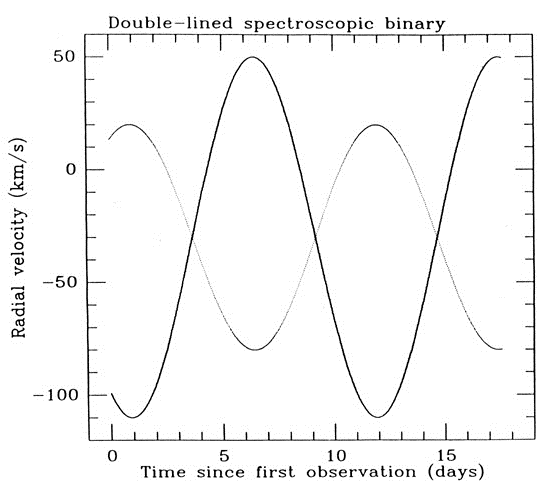
\includegraphics[scale=0.75]{2_ds}
\par\end{centering}

\end{figure}


\vspace{0.1in}

\begin{enumerate}
\item Label on the graph which curve is for the more massive star and which one is for the less massive star.

\begin{enumerate}
\item What is the radial velocity with respect to the Earth of the center of mass of the binary system?


\vspace{0.1in}



\rule[0.5pt]{0.15\paperwidth}{0.3pt} km/sec

\item Draw a horizontal line on the graph to indicate the radial velocity of the center of mass. Now estimate the maximum radial velocities of the two stars, relative to the center of mass.\vspace{0.1in}


\begin{enumerate}
\item more massive star, $K_{1}$ \rule[0.5pt]{0.1\paperwidth}{0.3pt} km/sec


\begin{center}
\vspace{0.1in}

\par\end{center}

\item less massive star, $K_{2}$ \rule[0.5pt]{0.1\paperwidth}{0.3pt} km/sec
\end{enumerate}
\end{enumerate}
\item From the exact sinusoidal nature of the radial velocity curve, what is the eccentricity of the orbit?

\begin{enumerate}
\item eccentricity $e=$ \rule[0.5pt]{0.1\paperwidth}{0.3pt}
\end{enumerate}
\item What is the period of the orbit? P = \rule[0.5pt]{0.1\paperwidth}{0.3pt} days


\vspace{0.1in}


\item Calculate the ratio of the masses. $\frac{m_{1}}{m_{2}}$ = \rule[0.5pt]{0.1\paperwidth}{0.3pt}


\pagebreak{}


\uline{\hspace{-0.4in}Lab \LabNumber ~~~~~~~~~~~~~~~~~~~~~~~~~~~~~~~~~~~~~~~~~~~~~~~~
Fall \year ~~~~~~~~~~~~~~~~~~~~~~~~~~~~~
Astro 1103 - Nature of the Universe}\vspace{0.3in}


\item Suppose that the system is also an eclipsing binary so $i=90^{\circ}$. We can use the equations given in the lab to derive the masses of the two stars and the orbit semimajor axis $a=a_{1}+a_{2}$.


First, we need to know the semimajor axis. Given the eccentricity of the system you can figure out $a_{1}$ and $a_{2}$ because you know the orbital period and the velocity. To help yourself, draw a picture of the ``top view'' of the orbit:


\vspace{2in}



Similar to above questions, determine what is the orbital velocity of:


\vspace{0.1in}

\begin{enumerate}
\item more massive star \rule[0.5pt]{0.05\paperwidth}{0.3pt} km/sec


\begin{center}
\vspace{0.1in}

\par\end{center}

\item less massive star \rule[0.5pt]{0.05\paperwidth}{0.3pt} km/sec


\begin{center}
\vspace{0.1in}

\par\end{center}

\end{enumerate}

Label $a_{1}$ and $a_{2}$ on the picture and indicate which star is the more massive.

\end{enumerate}
\vspace{0.1in}


You can now calculate the distances traveled by each star in its orbit, because you know what the orbit looks like, how fast the star travels, and how long it takes to make one orbit. Notice that the:

\vspace{0.1in}


Number of seconds in a day = 24 hrs $\times$ 60 $\frac{min}{hr}$ $\times$ 60 $\frac{sec}{min}$ = $8.64\times10^{4}$ sec/day

\vspace{0.1in}


Also, note that 1 AU = $1.50\times10^{8}$ km

\vspace{0.1in}


Now calculate $a_{1}$ and $a_{2}$ in AU. Show your calculation below. (HINT: speed = distance/time, so distance = speed $\times$ time.)

\begin{center}
\vspace{0.1in}
$a_{1}$ = \rule[0.5pt]{0.05\paperwidth}{0.3pt} AU
\par\end{center}

\begin{center}
\vspace{0.1in}
$a_{2}$ = \rule[0.5pt]{0.05\paperwidth}{0.3pt} AU
\par\end{center}

\begin{center}
Remember that, $a_{2}sin\,(i)=K_{2}$ , $a_{1}sin\,(i)=K_{1}$. The semimajor axis a is just the sum of $a_{1}+a_{2}$:
\par\end{center}

\begin{center}
\vspace{0.1in}
$a$ = \rule[0.5pt]{0.05\paperwidth}{0.3pt} AU
\par\end{center}

Calculate the sum of the masses (remember you need the period in years!) and then the separate masses (since you know the mass ratio).

\begin{center}
\vspace{0.1in}
P = \rule[0.5pt]{0.05\paperwidth}{0.3pt} years
\par\end{center}

\begin{center}
\vspace{0.1in}
$m_{1}+m_{2}$= \rule[0.5pt]{0.05\paperwidth}{0.3pt} $M_{\circledcirc}$
, $m_{1}$ = \rule[0.5pt]{0.05\paperwidth}{0.3pt} $M_{\circledcirc}$
, $m_{2}$ = \rule[0.5pt]{0.05\paperwidth}{0.3pt} $M_{\circledcirc}$
\par\end{center}
\end{document}
